% !TEX root = ../main.tex
\subsection{Markov Prefetcher}
\label{sec:markovPrefetcher}
The markov prefetcher, as described in \cite{Grannas}, is an address based prefetcher. It remembers past sequences of memory misses, and applies statistics to these sequences to predict future memory accesses.

As shown in \cite{Joseph}, it utilizes a graph with nodes representing cache blocks, and edges representing the probability that the connected node corresponds to the block being accessed next in the access sequence (see figure \ref{fig:markov}). The weight of the edges is determined by how often the cache block an edge points to is accessed directly after the node the edge is pointing from. For each memory access, the edge corresponding to the current transition needs to be updated. 

When predicting the next sequence of addresses, the markov prefetcher follows the best path through the graph. Configuring the markov prefetcher would allow you to decide how many addresses it should prefetch, when to create a new edge between two nodes, when to delete an edge and when to delete a node.

Looking at figure \ref{fig:markov}, if two addresses were to be prefetched, and \emph{0x0001} was the current node, then addresses \emph{0x0002} and \emph{0x0003} would be prefetched.

\begin{figure}[H]
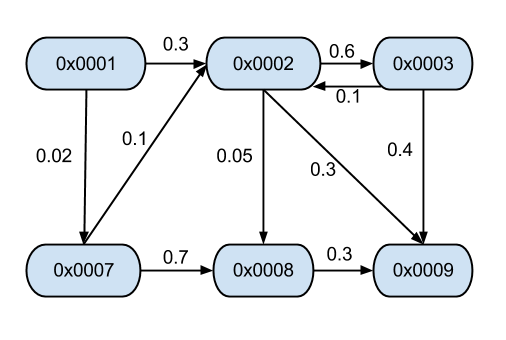
\includegraphics[scale=0.5]{./figures/markov}
\caption{\label{fig:markov}An illustration of the markov weighted graph}
\end{figure}

